\documentclass[12pt]{article}

\usepackage{amsmath}
\usepackage{amssymb}
\usepackage[dvips]{graphicx}
\usepackage{eepic}
\usepackage{color}
\usepackage{wasysym} % \female \male
\usepackage[landscape,pdftex]{geometry}
\usepackage{fancyhdr}
\usepackage{wasysym} % for check symbol



\DeclareOption{bigsym}{\DeclareSymbolFont{largesymbols}{OMX}{psycm}{m}{n}}
\ProcessOptions

\setlength{\oddsidemargin}{-0.75in}
\setlength{\evensidemargin}{-0.75in}
\setlength{\topmargin}{-1in}
\setlength{\textheight}{7.75in}
\setlength{\textwidth}{10.5in}
\setlength{\footskip}{0in}
\setlength{\parindent}{0pt}
\setlength{\rightskip}{0pt plus 1fil} % makes ragged right

\renewcommand{\familydefault}{phv} % helvetica

% following: color
\definecolor{mybgcolor}{rgb}{0.14,0.14,0.14}
\definecolor{myyellow}{rgb}{1,1,0.7}
\definecolor{myblue}{rgb}{0.4,0.8,1}
\definecolor{mydarkblue}{rgb}{0, 0.25, 0.5}
\definecolor{mypink}{rgb}{1,0.7,1}
\definecolor{myhotpink}{rgb}{1,0,0.6}
\definecolor{mywhite}{rgb}{1,1,1}

% following: B/W
%\definecolor{mybgcolor}{rgb}{1,1,1}
%\definecolor{myyellow}{rgb}{0,0,0}
%\definecolor{myblue}{rgb}{0,0,0}
%\definecolor{mypink}{rgb}{0,0,0}
%\definecolor{myhotpink}{rgb}{0,0,0}
%\definecolor{mywhite}{rgb}{0,0,0}

% header/footer layout
\pagestyle{fancy}
\lhead{} \chead{} \rhead{}
\lfoot{} \cfoot{} \rfoot{\color{myyellow} \thepage}
\renewcommand{\headrulewidth}{0pt}
\renewcommand{\footrulewidth}{0pt}

% font sizes
\newcommand{\superlarge}{\fontsize{60}{60} \selectfont}
\newcommand{\titlesize}{\fontsize{40}{50} \selectfont}
\newcommand{\headsize}{\fontsize{35}{35} \selectfont}
\newcommand{\textsize}{\fontsize{30}{35} \selectfont}
\newcommand{\smallsize}{\fontsize{25}{30} \selectfont}
\newcommand{\smallersize}{\fontsize{20}{25} \selectfont}
\newcommand{\smallestsize}{\fontsize{18}{22} \selectfont}
\newcommand{\evensmaller}{\fontsize{14}{18} \selectfont}
\newcommand{\lod}{\text{LOD}}
\newcommand{\bic}{\text{BIC}}
\newcommand{\rss}{\text{RSS}}
\newcommand{\var}{\text{var}}
\newcommand{\M}{\text{M}}
%\renewcommand{\log}{\text{log}}
%\renewcommand{\max}{\text{max}}



\pagecolor{mybgcolor}
\color{mywhite}

\begin{document}

\thispagestyle{empty}

\begin{center}
\titlesize \color{myyellow}

\vspace*{15mm}

{\headsize MAGIC design} \\
{\smallsize \color{myblue} and other topics}

\vspace*{5mm}

\color{mypink}
\rule{10in}{1mm}

\vspace*{20mm}

\smallsize
\color{white}
Karl Broman
\vspace{5mm}

\color{myblue}
{\smallersize Biostatistics \& Medical Informatics

University of Wisconsin -- Madison
\vspace{20mm}


\verb|biostat.wisc.edu/~kbroman|
}

\end{center}


\newpage
\thispagestyle{empty}

\vspace*{-0.85in}

\centerline{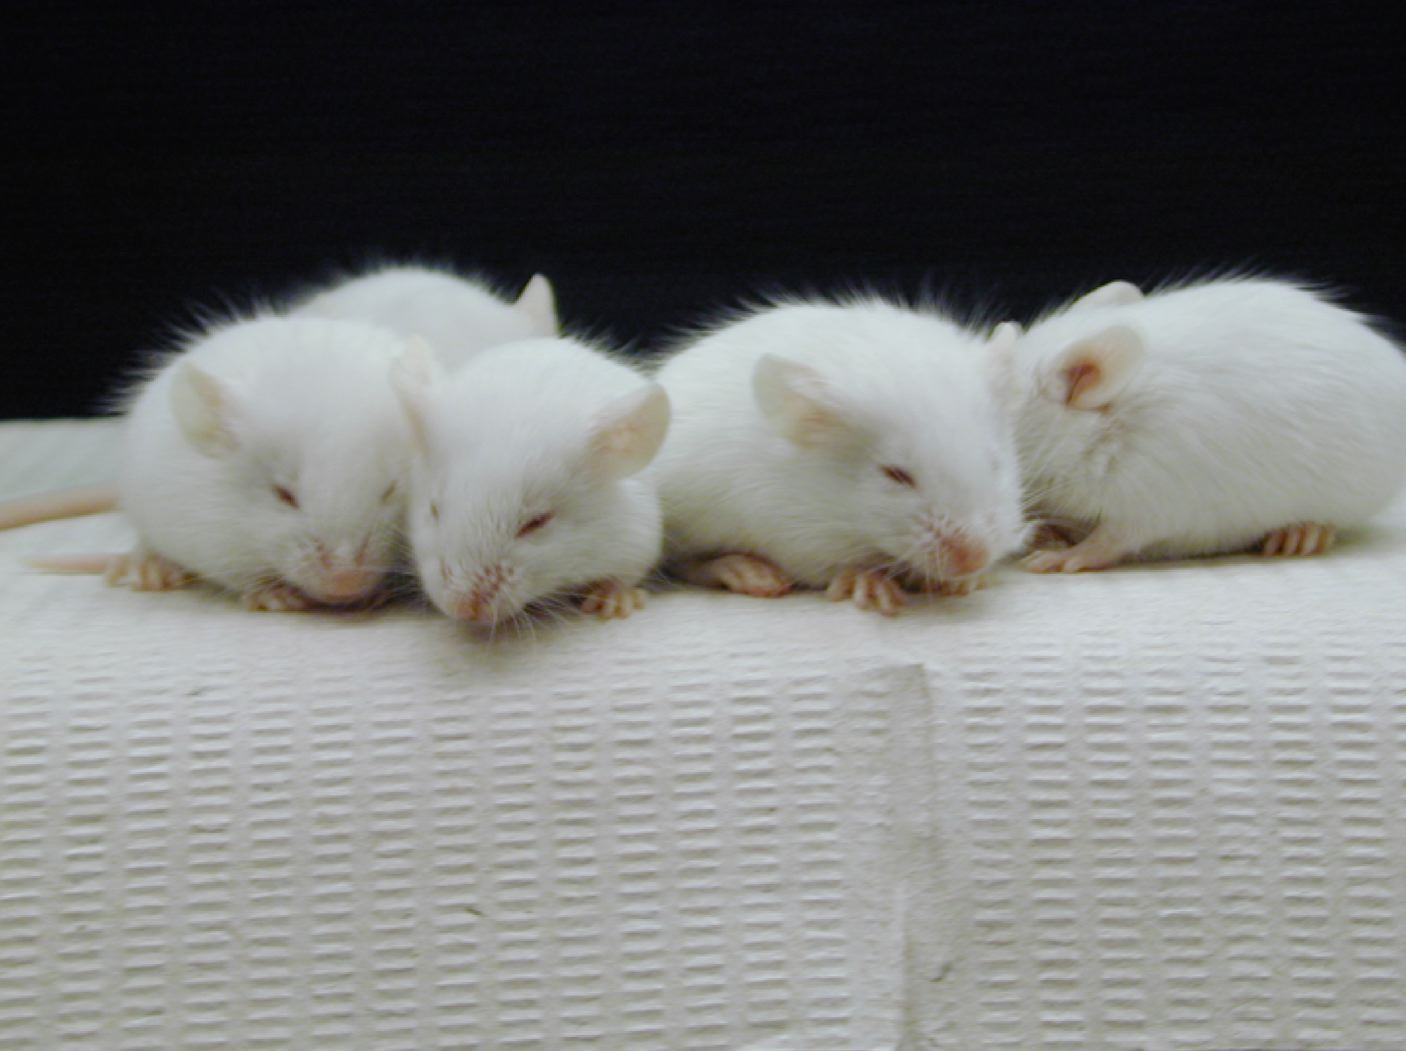
\includegraphics[height=9in]{Figs/inbredmice.jpg}}


\newpage

\headsize \color{myyellow}
\hfill \begin{minipage}{5.75in}
\centering
MAGIC lines
\end{minipage}

\vspace{20mm}

\centerline{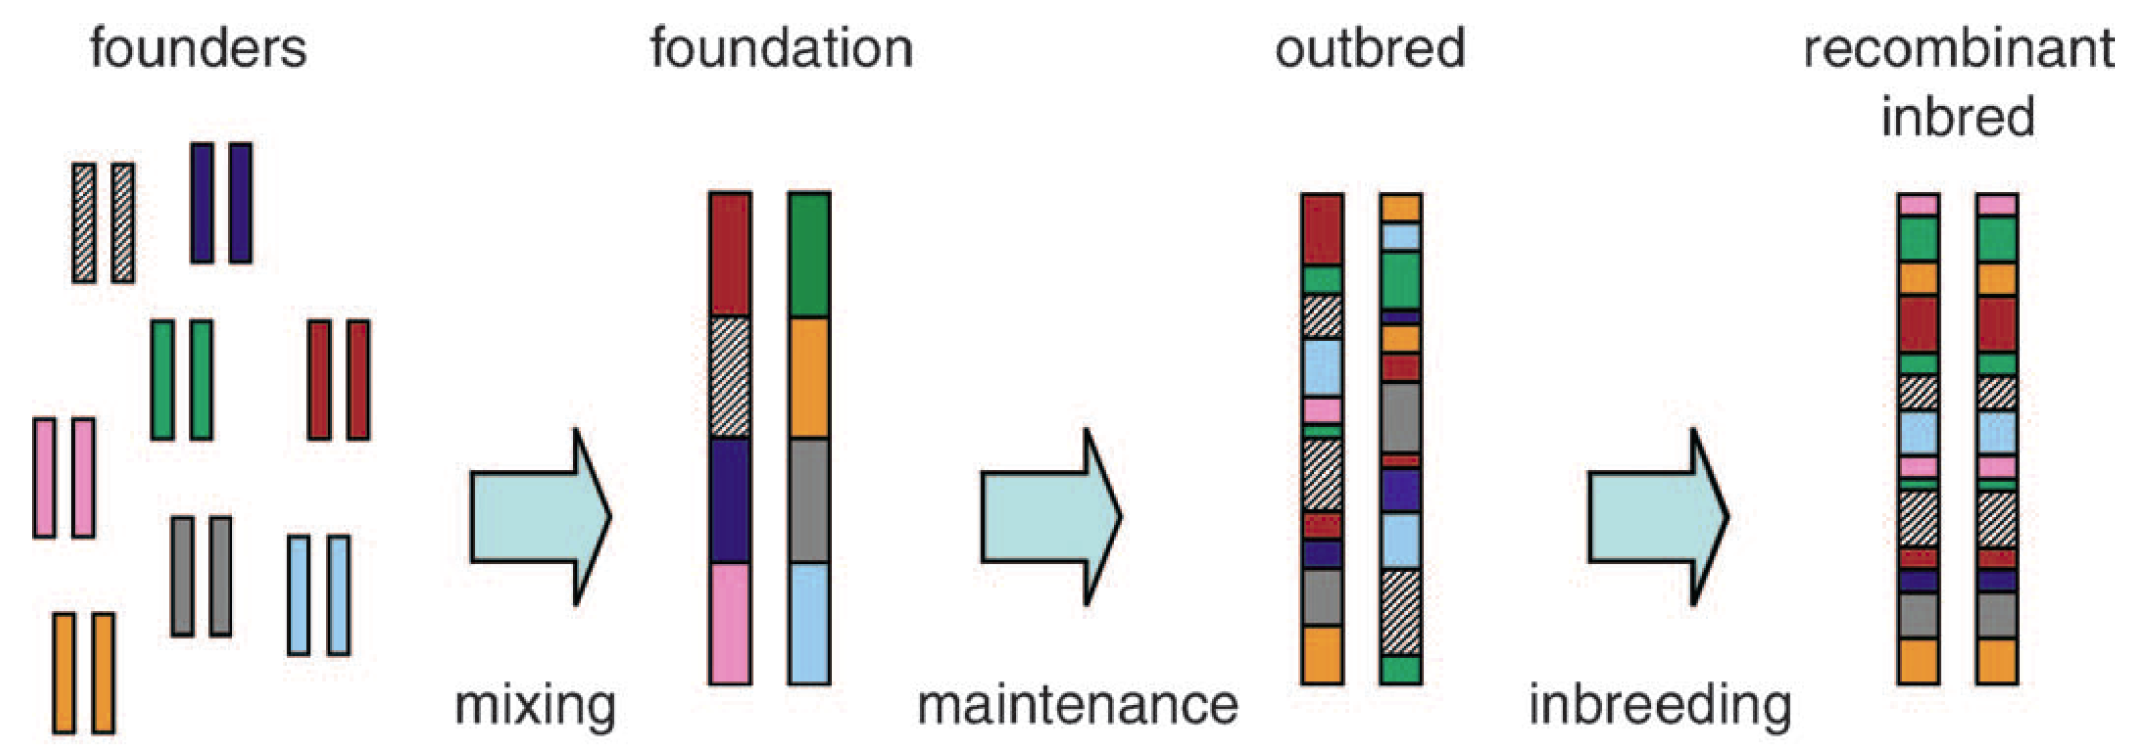
\includegraphics[width=10in]{Figs/valdar_genet2006.png}}

\vfill

\hfill {\smallestsize \color{myblue} Valdar et al. (2006) Genetics}

\vspace*{5mm}


\newpage

\addtocounter{page}{-1}

\headsize \color{myyellow}
\hfill \begin{minipage}{5.75in}
\centering
MAGIC lines
\end{minipage}

\vspace{20mm}

\centerline{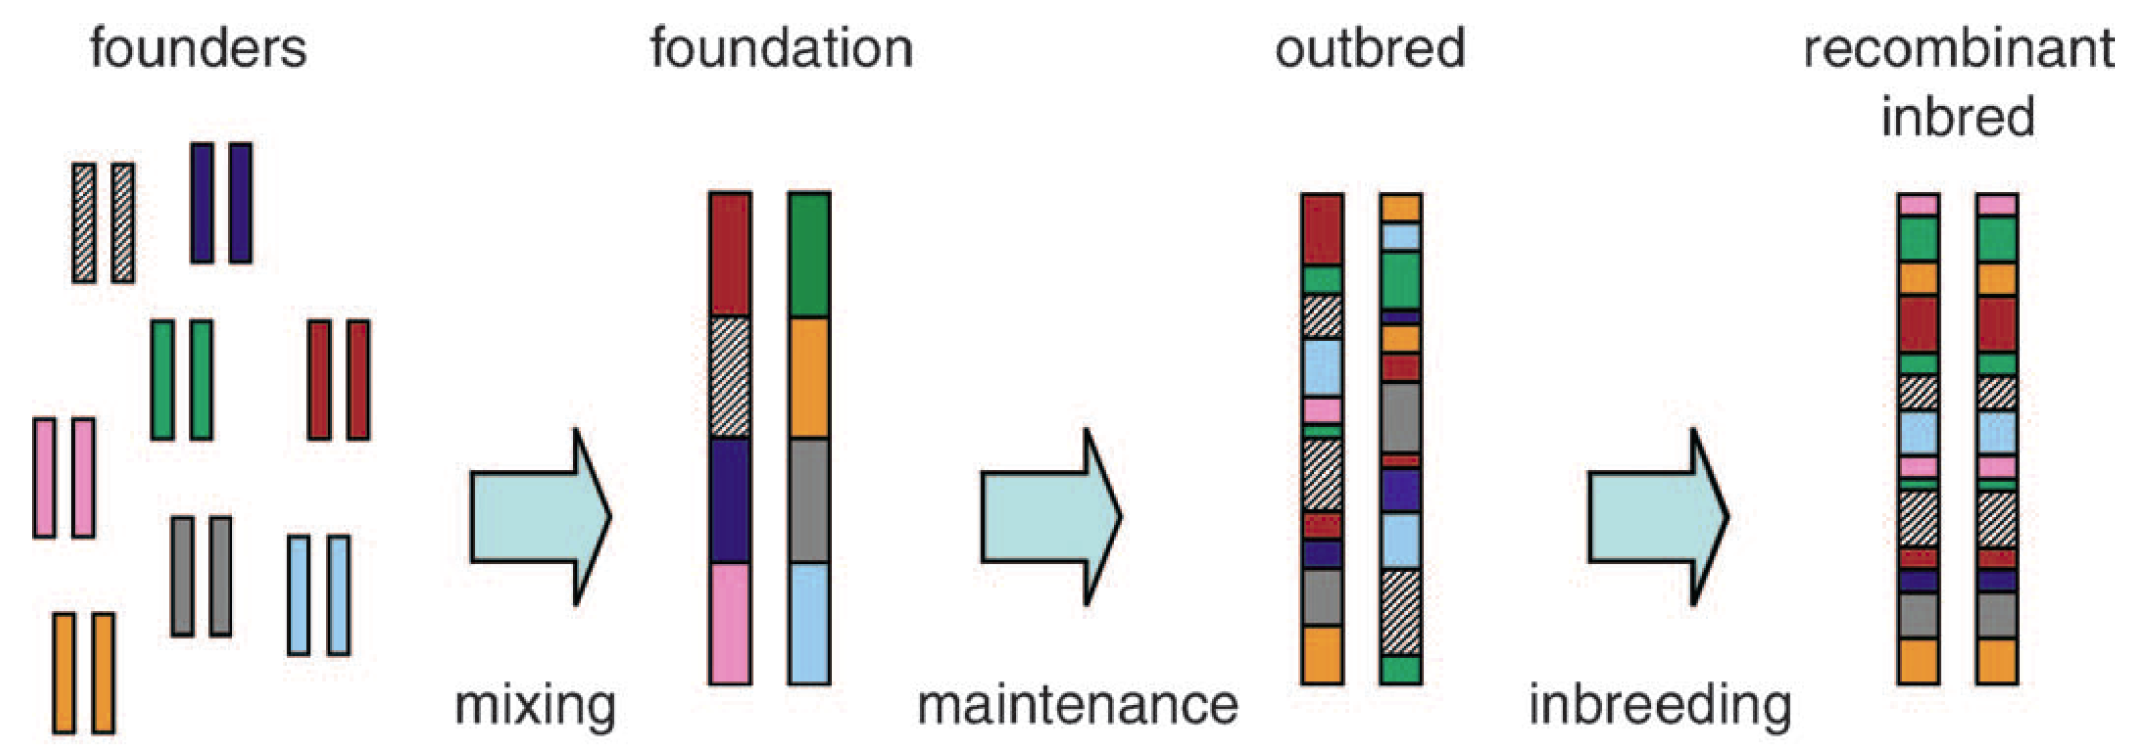
\includegraphics[width=10in]{Figs/valdar_genet2006.png}}

\smallsize \color{myyellow}
\hspace*{52mm} combine \hspace*{35mm} mix \hspace*{52mm} fix

\vfill

\hfill {\smallestsize \color{myblue} Valdar et al. (2006) Genetics}

\vspace*{5mm}


\newpage

\addtocounter{page}{-1}

\headsize \color{myyellow}
\hfill \begin{minipage}{5.75in}
\centering
MAGIC lines
\end{minipage}

\vspace{20mm}

\centerline{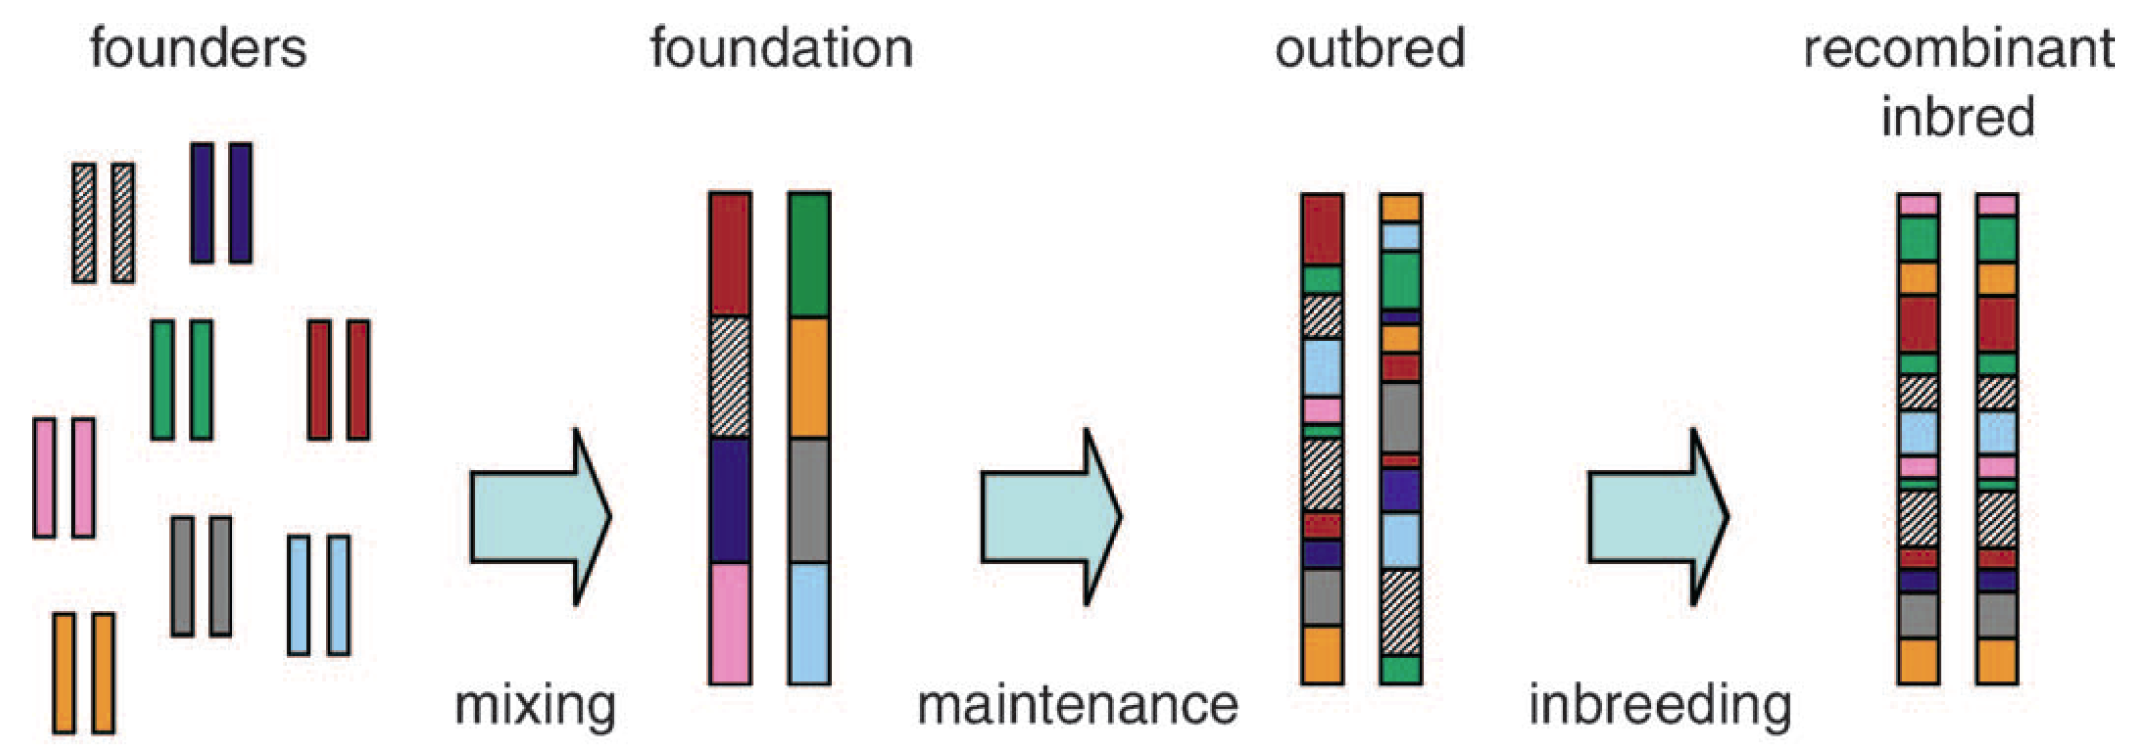
\includegraphics[width=10in]{Figs/valdar_genet2006.png}}

\smallsize \color{myyellow}
\hspace*{52mm} combine \hspace*{35mm} mix \hspace*{52mm} fix

\smallersize
\color{mywhite}
\vspace{20pt}

\hspace*{6mm}
\begin{minipage}[t]{45mm}
\vspace*{0mm}
\centering

How many? \\[20pt]

\end{minipage}
\hspace{57mm}
\begin{minipage}[t]{45mm}
\vspace*{0mm}
\centering


\end{minipage}
\hspace{18mm}
\begin{minipage}[t]{45mm}
\vspace*{0mm}
\centering


\end{minipage}


\vfill

\hfill {\smallestsize \color{myblue} Valdar et al. (2006) Genetics}

\vspace*{5mm}


\newpage

\addtocounter{page}{-1}

\headsize \color{myyellow}
\hfill \begin{minipage}{5.75in}
\centering
MAGIC lines
\end{minipage}

\vspace{20mm}

\centerline{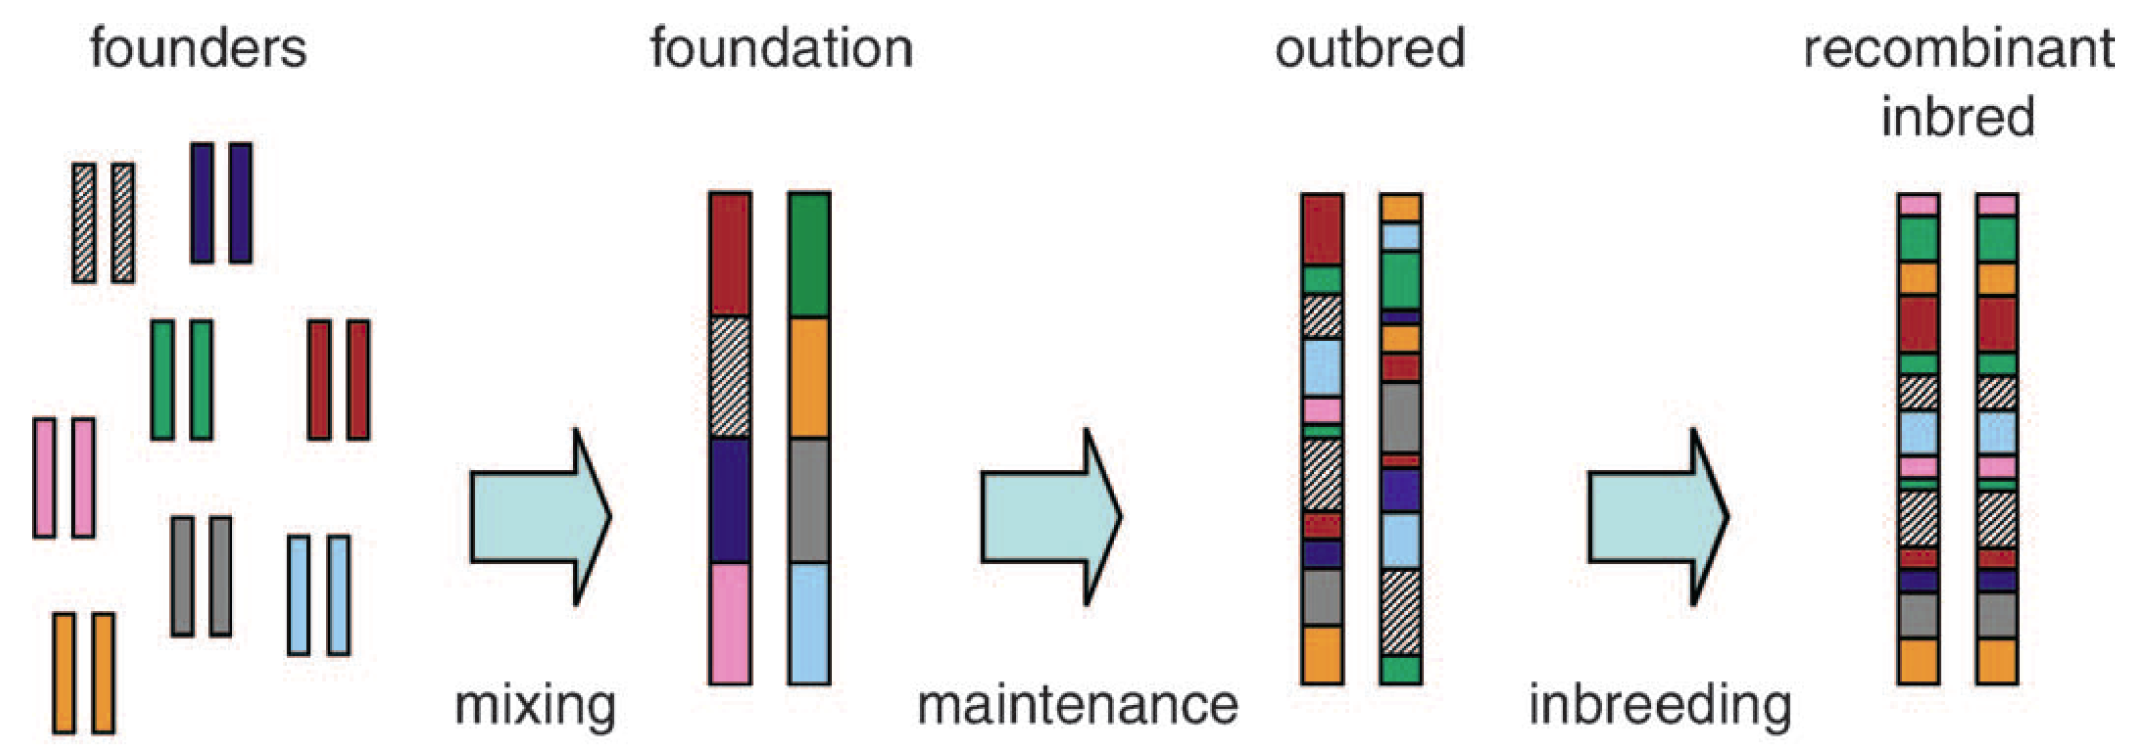
\includegraphics[width=10in]{Figs/valdar_genet2006.png}}

\smallsize \color{myyellow}
\hspace*{52mm} combine \hspace*{35mm} mix \hspace*{52mm} fix

\smallersize
\color{mywhite}
\vspace{20pt}

\hspace*{6mm}
\begin{minipage}[t]{45mm}
\vspace*{0mm}
\centering

How many? \\[20pt]
Which?
\end{minipage}
\hspace{57mm}
\begin{minipage}[t]{45mm}
\vspace*{0mm}
\centering

\end{minipage}
\hspace{18mm}
\begin{minipage}[t]{45mm}
\vspace*{0mm}
\centering


\end{minipage}


\vfill

\hfill {\smallestsize \color{myblue} Valdar et al. (2006) Genetics}

\vspace*{5mm}


\newpage

\addtocounter{page}{-1}

\headsize \color{myyellow}
\hfill \begin{minipage}{5.75in}
\centering
MAGIC lines
\end{minipage}

\vspace{20mm}

\centerline{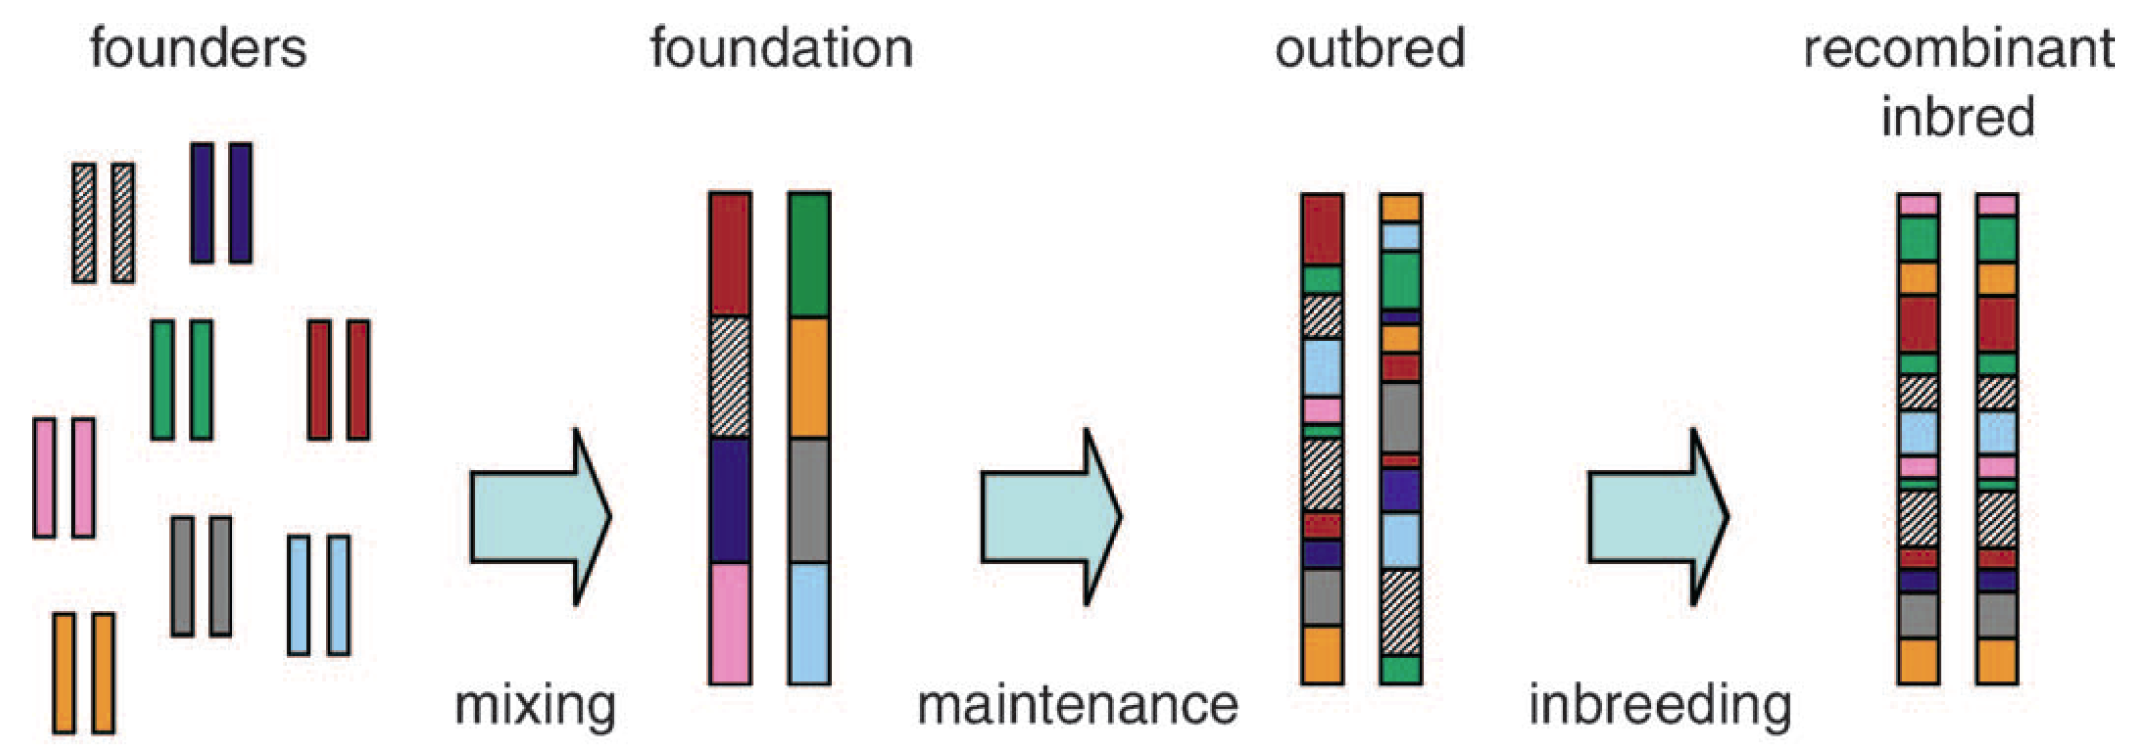
\includegraphics[width=10in]{Figs/valdar_genet2006.png}}

\smallsize \color{myyellow}
\hspace*{52mm} combine \hspace*{35mm} mix \hspace*{52mm} fix

\smallersize
\color{mywhite}
\vspace{20pt}

\hspace*{6mm}
\begin{minipage}[t]{45mm}
\vspace*{0mm}
\centering

How many? \\[20pt]
Which?
\end{minipage}
\hspace{57mm}
\begin{minipage}[t]{45mm}
\vspace*{0mm}
\centering

How long?
\end{minipage}
\hspace{18mm}
\begin{minipage}[t]{45mm}
\vspace*{0mm}
\centering


\end{minipage}


\vfill

\hfill {\smallestsize \color{myblue} Valdar et al. (2006) Genetics}

\vspace*{5mm}


\newpage

\addtocounter{page}{-1}

\headsize \color{myyellow}
\hfill \begin{minipage}{5.75in}
\centering
MAGIC lines
\end{minipage}

\vspace{20mm}

\centerline{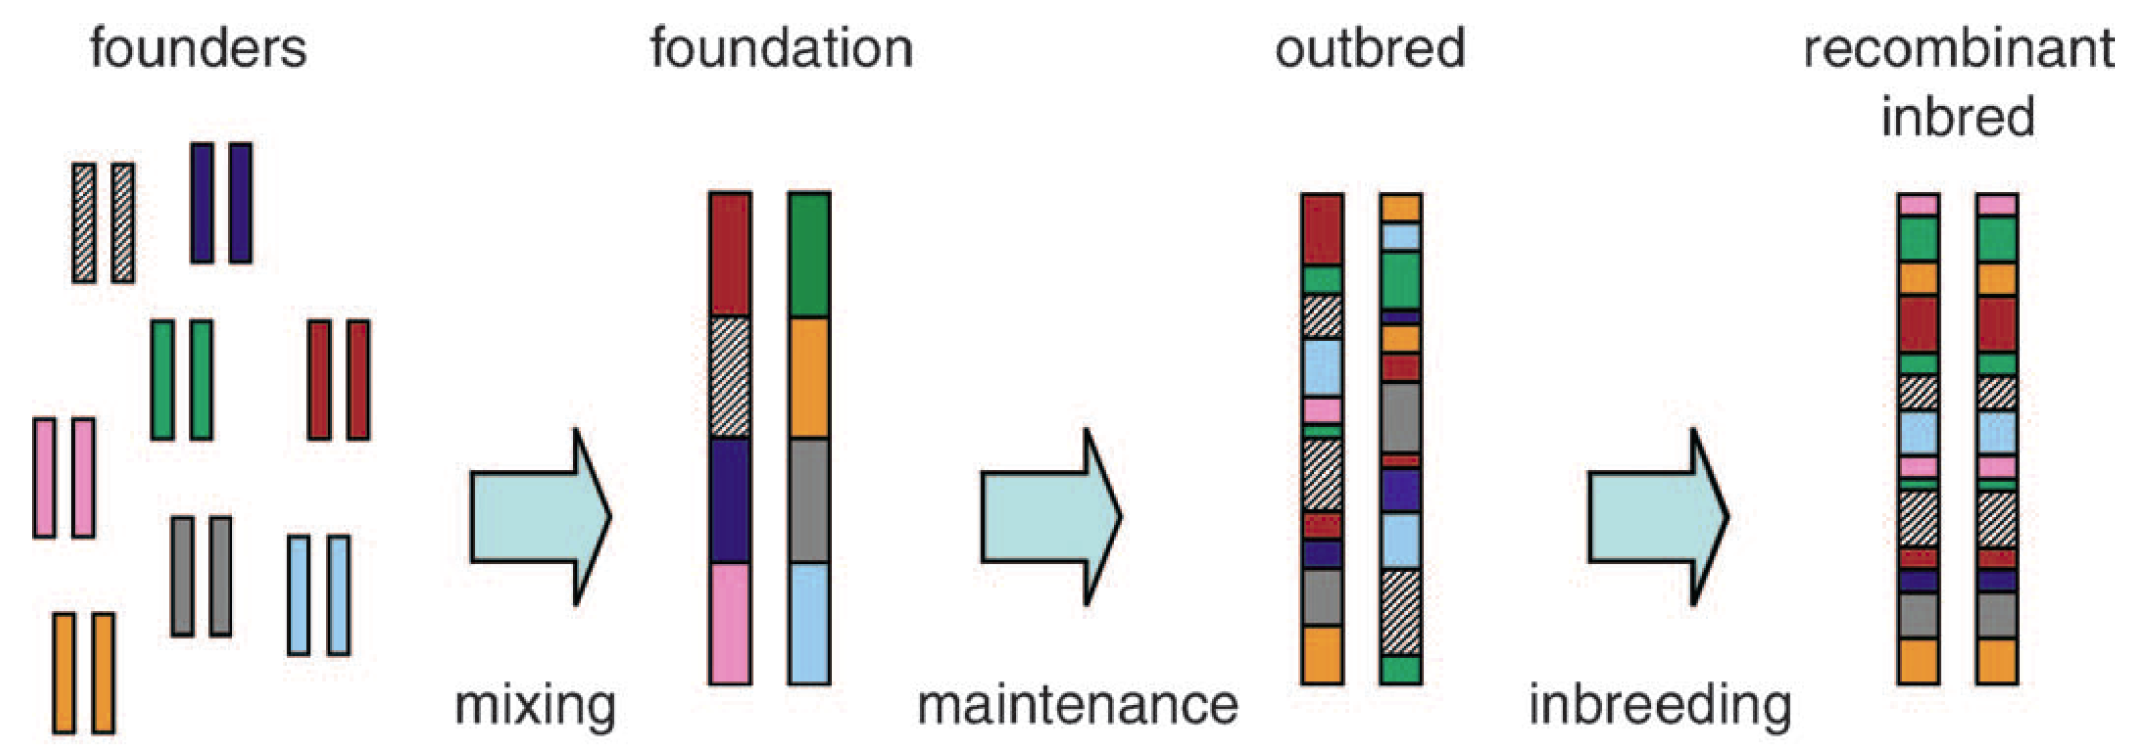
\includegraphics[width=10in]{Figs/valdar_genet2006.png}}

\smallsize \color{myyellow}
\hspace*{52mm} combine \hspace*{35mm} mix \hspace*{52mm} fix

\smallersize
\color{mywhite}
\vspace{20pt}

\hspace*{6mm}
\begin{minipage}[t]{45mm}
\vspace*{0mm}
\centering

How many? \\[20pt]
Which?
\end{minipage}
\hspace{57mm}
\begin{minipage}[t]{45mm}
\vspace*{0mm}
\centering

How long?
\end{minipage}
\hspace{18mm}
\begin{minipage}[t]{45mm}
\vspace*{0mm}
\centering

How?
\end{minipage}


\vfill

\hfill {\smallestsize \color{myblue} Valdar et al. (2006) Genetics}

\vspace*{5mm}


\newpage

\headsize \color{myyellow}
\hfill \begin{minipage}{5.75in}
\centering
But first \dots
\end{minipage}

\vfill

\centerline{\includegraphics{Figs/ri8.pdf}}


\newpage

\headsize \color{myyellow}
\hfill \begin{minipage}{5.75in}
\centering
Simulation results
\end{minipage}

\vfill

\centerline{\includegraphics{Figs/rf_by_sim.pdf}}

\vspace{15mm}

\newpage

\headsize \color{myyellow}
\hfill 
\begin{minipage}{6.55in}
\centering
Haldane \& Waddington 1931
\end{minipage}

\vfill

\centerline{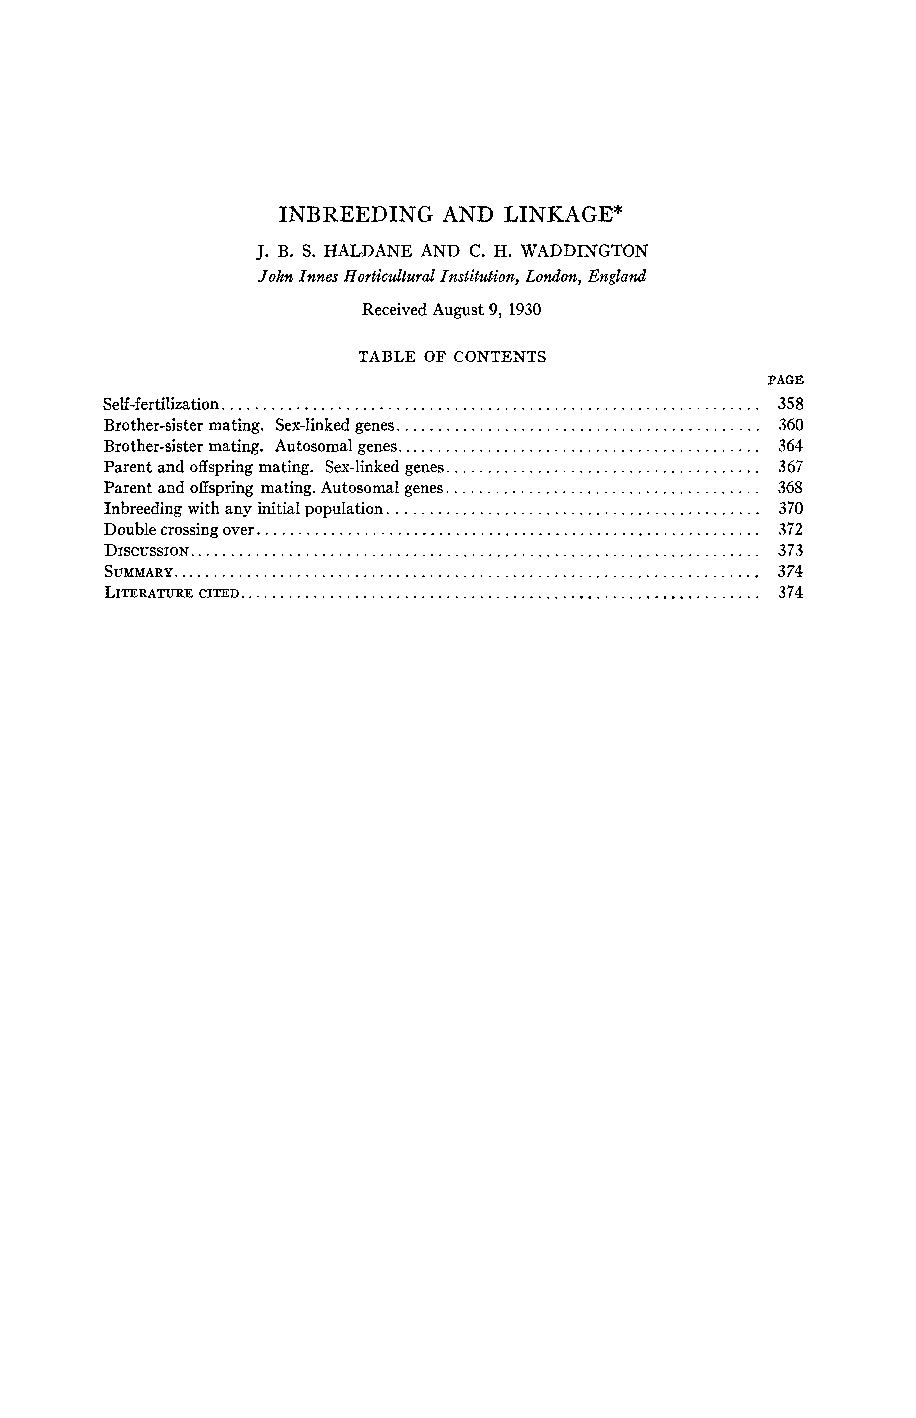
\includegraphics[width=10in]{Figs/haldane_title.pdf}}

\vspace{15mm}

\newpage

\headsize \color{myyellow}
\hfill 
\begin{minipage}{5.75in}
\centering
Result for selfing
\end{minipage}

\vfill

\centerline{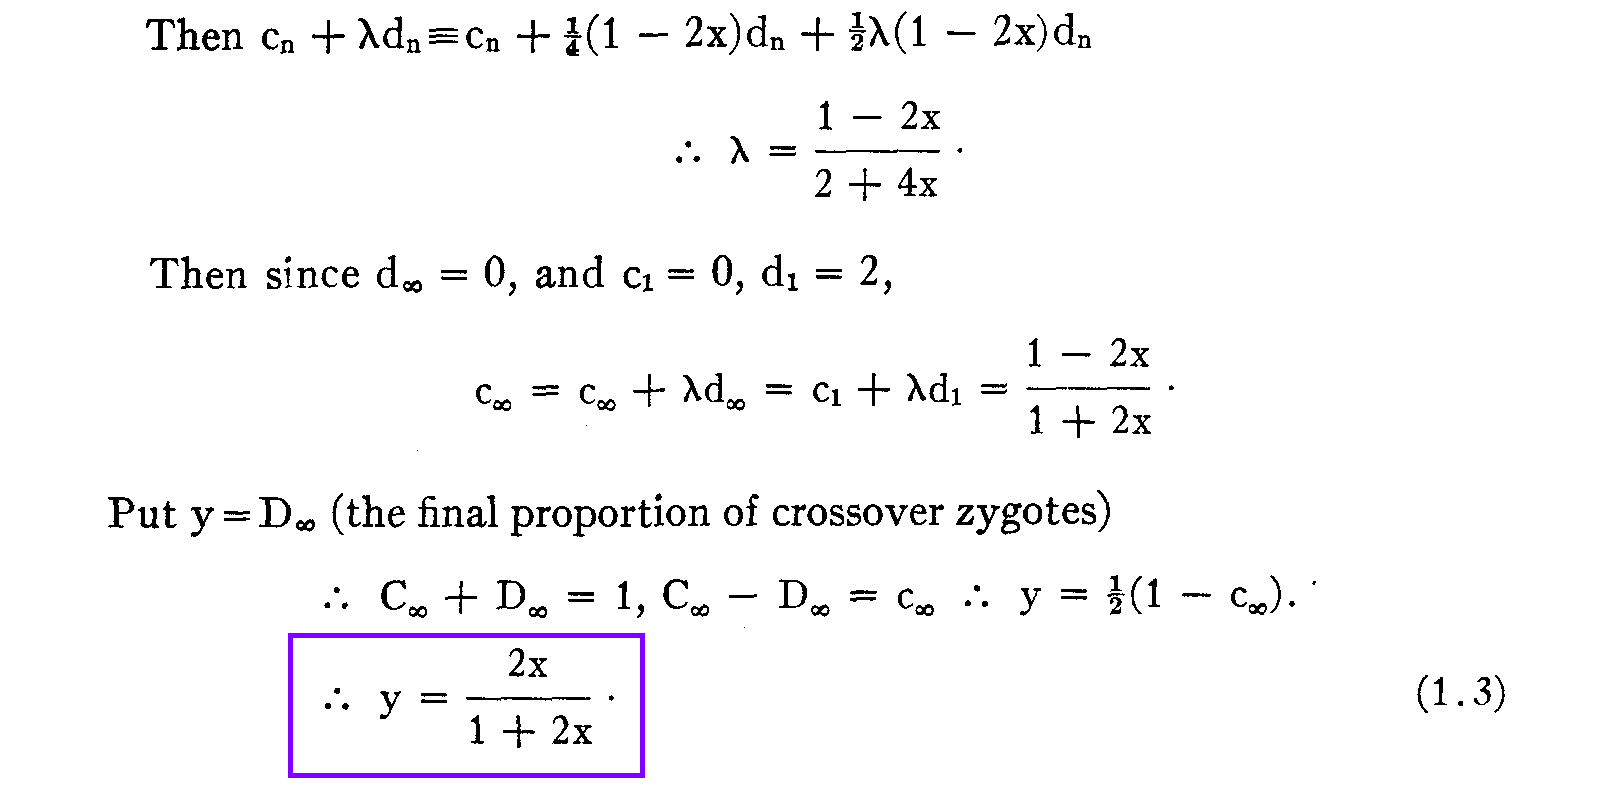
\includegraphics[width=10in]{Figs/haldane_selfing.png}}

\vspace{30mm}

\newpage
\headsize \color{myyellow}
\hfill 
\begin{minipage}{5.75in}
\centering
Result for sib-mating
\end{minipage}

\vfill

\centerline{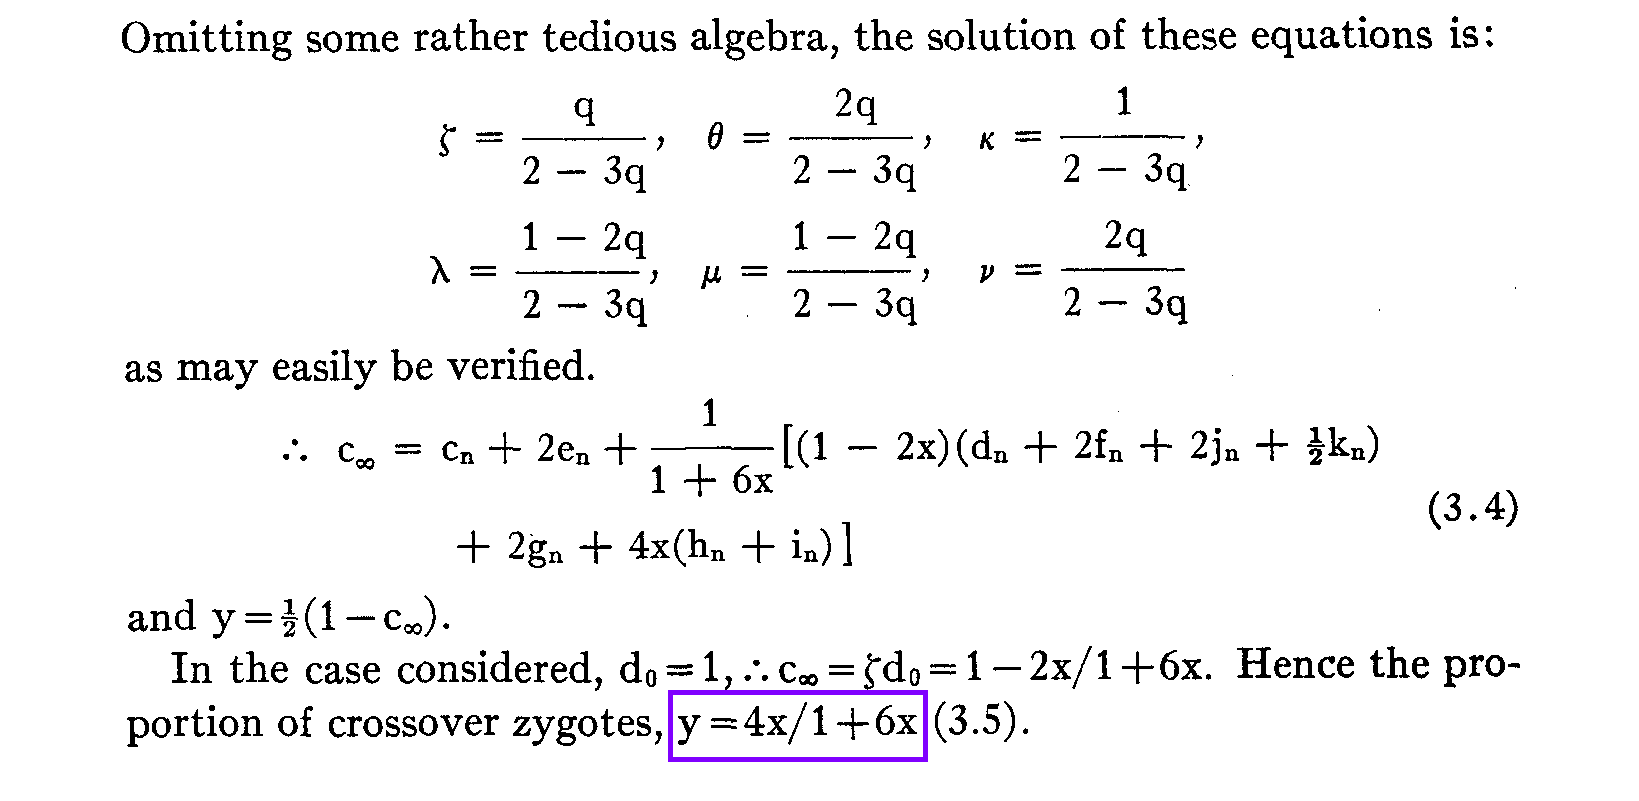
\includegraphics[width=10in]{Figs/haldane_sibmating3.png}}

\vspace{30mm}




\newpage

\headsize \color{myyellow}
\hfill \begin{minipage}{5.75in}
\centering
Simulation results
\end{minipage}

\vfill

\centerline{\includegraphics{Figs/rf_by_sim.pdf}}

\vspace{15mm}

\newpage

\headsize \color{myyellow}
\hfill \begin{minipage}{5.75in}
\centering
Simulation results
\end{minipage}

\vfill

\centerline{\includegraphics{Figs/rf_by_sim_genformula.pdf}}

\vspace{15mm}

\newpage

\headsize \color{myyellow}
\hfill \begin{minipage}{5.75in}
\centering
Non-linear regression
\end{minipage}


\vspace{30mm}

\textsize 
{\color{myblue}
\verb|      out <- nls(| {\tt \color{mypink} R \verb|~| a*r/(1 + b*r)}\verb|,| \\
\verb|                 data = data.frame(r=r, R=R),| \\
\verb|                 start = list(a=4, b=6))| \\
\verb|      summary(out)|
}

\newpage
\addtocounter{page}{-1}

\headsize \color{myyellow}
\hfill \begin{minipage}{5.75in}
\centering
Non-linear regression
\end{minipage}


\vspace{30mm}

\textsize 
{\color{myblue}
\verb|      out <- nls(| {\tt \color{mypink} R \verb|~| a*r/(1 + b*r)}\verb|,| \\
\verb|                 data = data.frame(r=r, R=R),| \\
\verb|                 start = list(a=4, b=6))| \\
\verb|      summary(out)|
}

\vspace{15mm}

\color{mywhite}
\verb|                            | \\
\verb|        Estimate  Std. Error| \\
\verb|      a    7.016       0.011| \\
\verb|      b    6.023       0.016|

\newpage
\addtocounter{page}{-1}

\headsize \color{myyellow}
\hfill \begin{minipage}{5.75in}
\centering
Non-linear regression
\end{minipage}


\vspace{30mm}

\textsize 
{\color{myblue}
\verb|      out <- nls(| {\tt \color{mypink} R \verb|~| a*r/(1 + b*r)}\verb|,| \\
\verb|                 data = data.frame(r=r, R=R),| \\
\verb|                 start = list(a=4, b=6))| \\
\verb|      summary(out)|
}

\vspace{15mm}

\color{mypink}
\verb|                                        More data       | \\
\color{mywhite}
\verb|        Estimate  Std. Error        Estimate  Std. Error| \\
\verb|      a    7.016       0.011      a    7.003       0.008| \\
\verb|      b    6.023       0.016      b    6.005       0.012|


\newpage

\headsize \color{myyellow}
\hfill \begin{minipage}{5.75in}
\centering
Simulation results
\end{minipage}

\vfill

\centerline{\includegraphics{Figs/rf_by_sim_moredata.pdf}}

\vspace{15mm}

\newpage

\headsize \color{myyellow}
\hfill \begin{minipage}{5.75in}
\centering
R/qtl
\end{minipage}

\vfill

\centerline{\includegraphics{Figs/rqtl_lines_code.pdf}}

\vspace{15mm}


\end{document}
